\chapter{Resultados}
\label{cap:results}

\section{RQ1. Com que frequência \textit{breaking changes} surgem \filipe{afetam? impactam?} nos pacotes clientes?}

Nesta Seção, encontram-se os resultados da análise manual voltados para responder a primeira questão de pesquisa. Nessa Seção estão os dados relacionados à quantificação das \textit{break changes}.

\subsubsection{Relação das \textit{releases} do cliente com os provedores e as \textit{breaking changes}}
\filipe{A primeira frase do primeiro parágrafo dos ``Resultados'' que eu esperava ler é algo do tipo: ``X\% das releases de pacotes clientes apresentam um defeito devido a uma breaking change.''. A primeira frase do segundo parágrafo eu esperava que fosse algo do tipo ``Y\% das releases dos pacotes do provedor causam uma breaking change em pelo menos um pacote cliente.'' Nesse momento está difícil orquestrar os resultados ...}
Após a análise manual em cada uma das \textit{releases} que resultaram em erro, foi constatado um total de 39 (10.15\%) pacotes que foram impactados por \textit{breaking changes}. \filipe{Agora sim ... fácil entender e responde à RQ!} Esses pacotes sofreram com \textit{breaking changes} em pelo menos uma de suas \textit{releases}. Desde pacotes com uma \textit{release} executada, até os pacotes com mais de 100 \textit{releases} executadas foram impactados e, de maneira análoga, pacotes com 1 provedor até pacotes com mais de 100 provedores também foram afetados por \textit{break changes}. \filipe{Certo ... mas aqui você poderia me dizer qual a correlação entre o número de releases afetadas por uma breaking change e o número de releases e provedores. Acredito que exista alguma correlação.} Assim sendo, o fator determinante para a manifestação de uma \textit{break change} não é apenas o tamanho do pacote cliente, nem tão pouco a quantidade de provedores que esse pacote possui. \filipe{Não sei se você pode dizer isso sem ao menos descrever essa correlação!}

A proporção com o qual o pacote foi atingido \filipe{impactado? use sempre a mesma palavra (corrija no resto do texto), eu prefiro impactado} também é um ponto importante a se considerar. Realizar a análise dos pacotes sem considerar o impacto que as \textit{break changes} causaram, não é justo. Por exemplo, o pacote \textit{assetgraph-builder}\footnote{https://www.npmjs.com/package/assetgraph-builder} possui 140 \textit{releases} que foram executadas, resultando em 23 (16.4\%) \textit{releases} que foram impactadas por \textit{breaking changes}. Já o pacote \textit{ember-cli-chartjs}\footnote{https://www.npmjs.com/package/ember-cli-chartjs}, que contém 7 \textit{releases} que foram executadas, resultou em 6 (85.7\%) \textit{releases} com \textit{breaking changes}. Essa discrepância no percentual ocorre pois a quantidade de \textit{break changes} não está somente relacionada com a quantidade de  \textit{releases} que esses pacotes contêm, mas também está relacionada com os provedores, uma vez que eles também influenciam na manifestação de uma \textit{break change}, pois são eles os causadores. \filipe{Mostre uma scatterplot com o número total de releases vs. a proporção de releases impactada por uma breaking change}

Uma análise mais justa se encontra no gráfico de dispersão da Figura \ref{fig:result_rq1_releases_affecteds}, que compara a quantidade de \textit{releases} com a quantidade de provedores. Nessa Figura estão dispersos todos pacotes da amostra e, em destaque, os que sofreram com \textit{break changes}. O eixo \textit{y} contém a variável do tamanho dos pacotes \filipe{O eixo y denota a quantidade de releases do pacote}, ou seja, a quantidade de \textit{releases} dos pacotes que foram executadas e que estavam sujeitas ao surgimento das \textit{break changes} \filipe{Tamanho não é uma boa palavra para quantidade de releases. Tamém não precisa dizer ``que foram executadas'' (executar uma release é estranho ...), pois você executou os testes de todas as releases, certo?}. Já no eixo \textit{x}, há a quantidade de provedores que esses pacotes possuem. Por fim, os  círculos, que simbolizam os pacotes, representam a proporção do pacote que foi afetado, ou seja, a quantidade de \textit{releases} afetadas pela quantidade de \textit{releases} executadas, assim, quanto maior os círculos vermelhos, maior o impacto da \textit{break change} nos pacotes por eles representados. \filipe{Não tem legenda para o tamanho dos círculos, difícil saber a proporção. Por que não colocar a proporção no eixo x e a quantidade de releases no eixo y? Outra coisa: essa análise deveria ser feita para o número de clientes também, ou não?} Os círculos cinzas representam os pacotes que não sofreram com \textit{break changes} e por isso possuem os mesmos tamanhos. Por fim, as linhas verdes interceptam os eixos na posição 15.

\begin{figure}
    \centering
    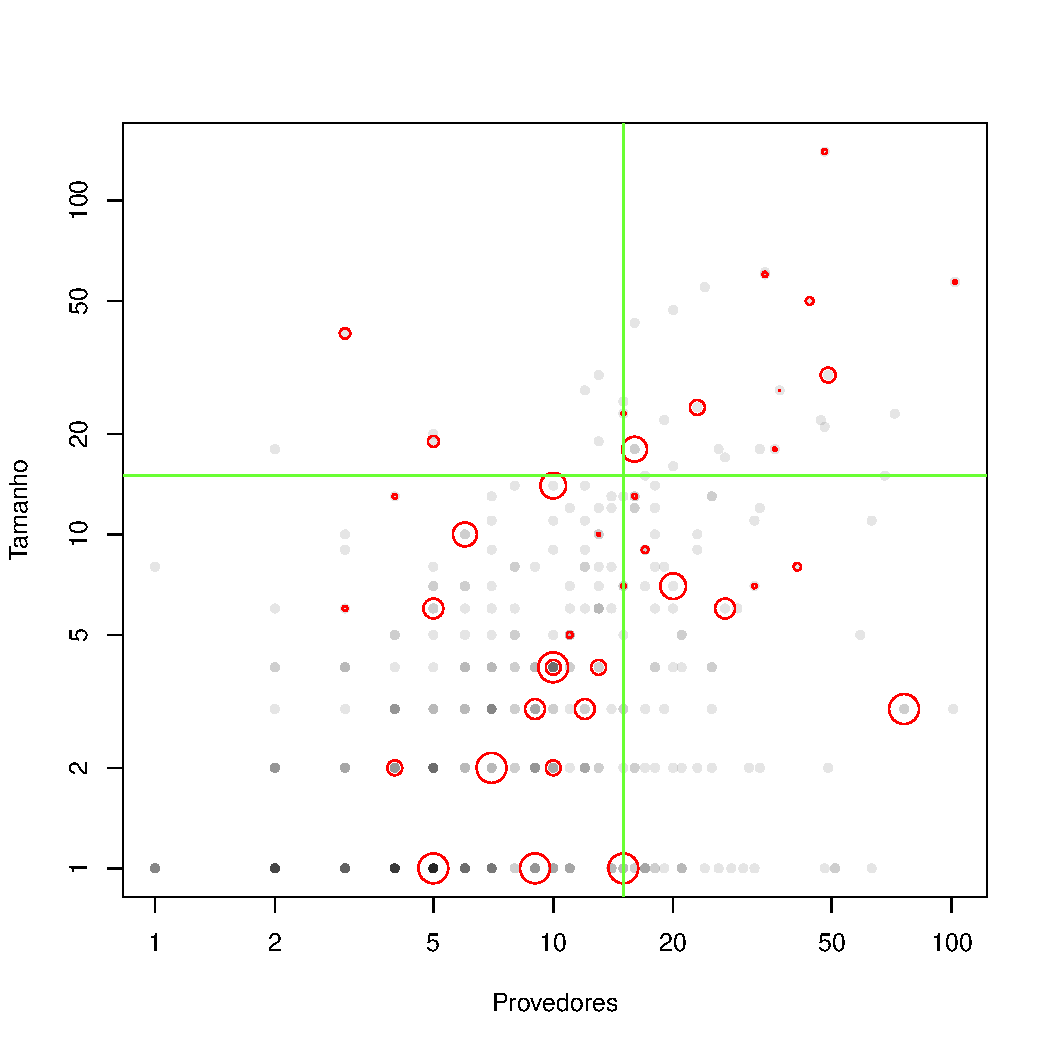
\includegraphics[scale=0.5]{figuras/result_rq1_releases_affecteds.pdf}
    \caption{Dispersão das \textit{break changes} em função do tamanho do pacote e a quantidade de provedores}
    \label{fig:result_rq1_releases_affecteds}
\end{figure}{}

Na Figura \ref{fig:result_rq1_releases_affecteds} pode-se perceber inicialmente que a quantidade de \textit{releases} executadas do cliente (eixo \textit{y}) não é um fator determinante para o surgimento de \textit{break changes}. Isso é um fato pois há uma concentração maior dos pacotes afetados que possuem menos de 15 \textit{releases} do que os pacotes afetados com mais que 15. Já os pacotes grandes, ou os com mais de 15 \textit{releases}, são mais impactados a medida que o número de provedores aumenta, pois a concentração de pacotes grandes com mais de 15 provedores é maior do que os com menos. Isso acontece pois quanto mais provedores um pacote tiver, maior é a chance do pacote ser impactado. \filipe{Ótimo!}

Um ponto interessante sobre os pacotes afetados é que, mesmo que possuam mais \textit{releases} e mais provedores que a média, a proporção afetada do pacote é baixa, ou seja, são poucas as \textit{releases} que foram afetadas. Isso pode ser explicado pelo fato de serem pacotes grandes \filipe{mude ``grandes'' por ``com muitas releases''. Tamanho geralmente é associado a número de linhas de código}, possuem um grande número de \textit{releases} e, consequentemente, estarem sempre lançando \textit{releases} se recuperando das \textit{break changes} que os tenham atingidos, assim minimizando o impacto da mesma sobre o pacote.

% a baixa quantidade de amostras para os dois e três casos de break changes deixou esta conclusão um pouco estranha e meio "não-genérica"
\subsubsection{Variedade de \textit{break changes} nos pacotes}
As \textit{break changes} são imprevisíveis. Elas ocorrem independentemente uma das outras, ou seja, um pacote pode ser impactado com apenas um caso de \textit{break change}, mas também pode ser impactado com mais de um caso. E foi isso o que aconteceu: dos 39 pacotes afetados, 34 (87\%) foram impactados por apenas um caso de \textit{break change} e 5 (12.8\%) foram impactados por mais de um caso, sendo que 4 (10.2\%) foram impactados por dois casos e 1 (2.5\%) pacote sofreu a manifestação de 3 casos de \textit{break change}. A Figura \ref{fig:result_rq1_once_twice_three_1} contém estes dados.

\begin {figure} [h!]
   \centering
   \mbox {
        \subfigure[]{\label{fig:result_rq1_once_twice_three_1} 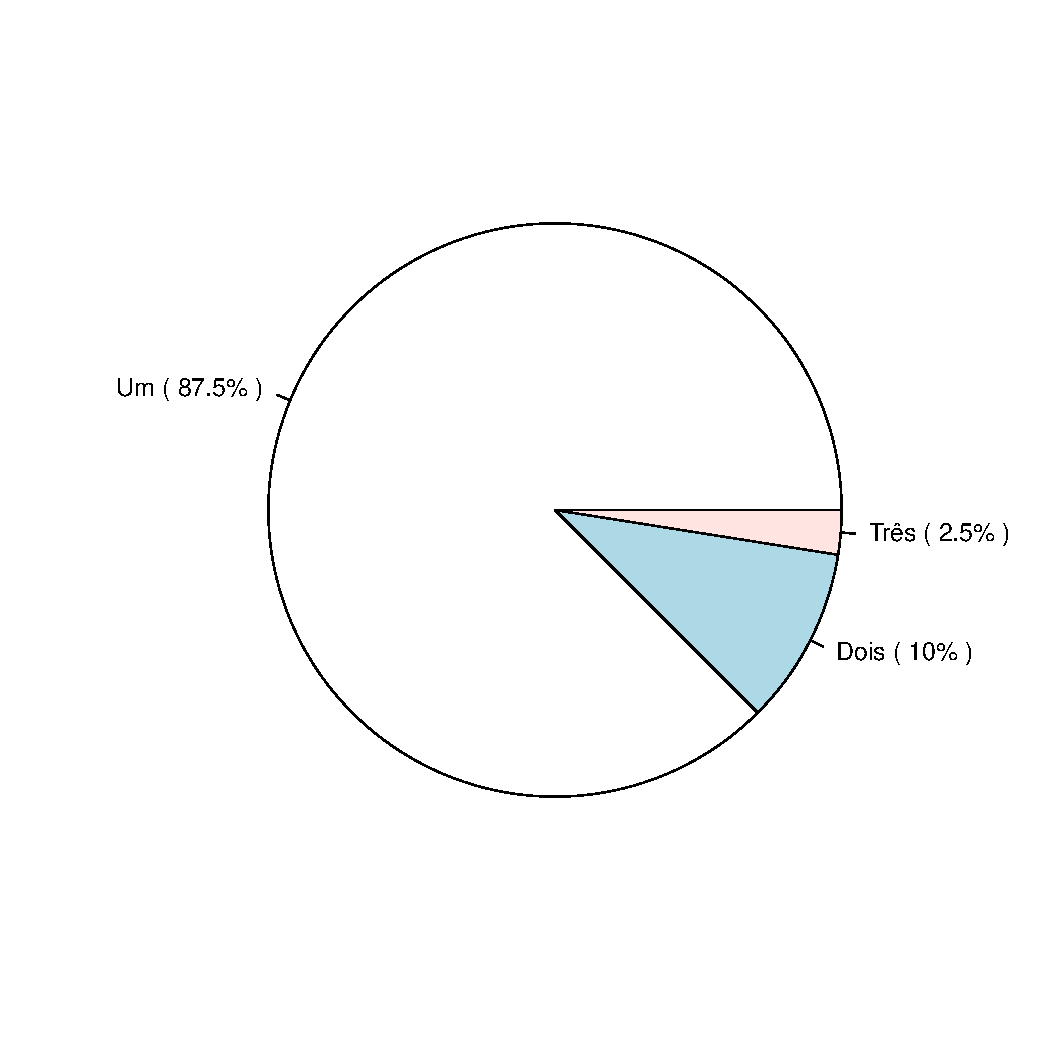
\includegraphics[scale=0.4]{figuras/result_rq1_once_twice_three_1.pdf}}\quad
        \subfigure[]{\label{fig:result_rq1_once_twice_three_2} 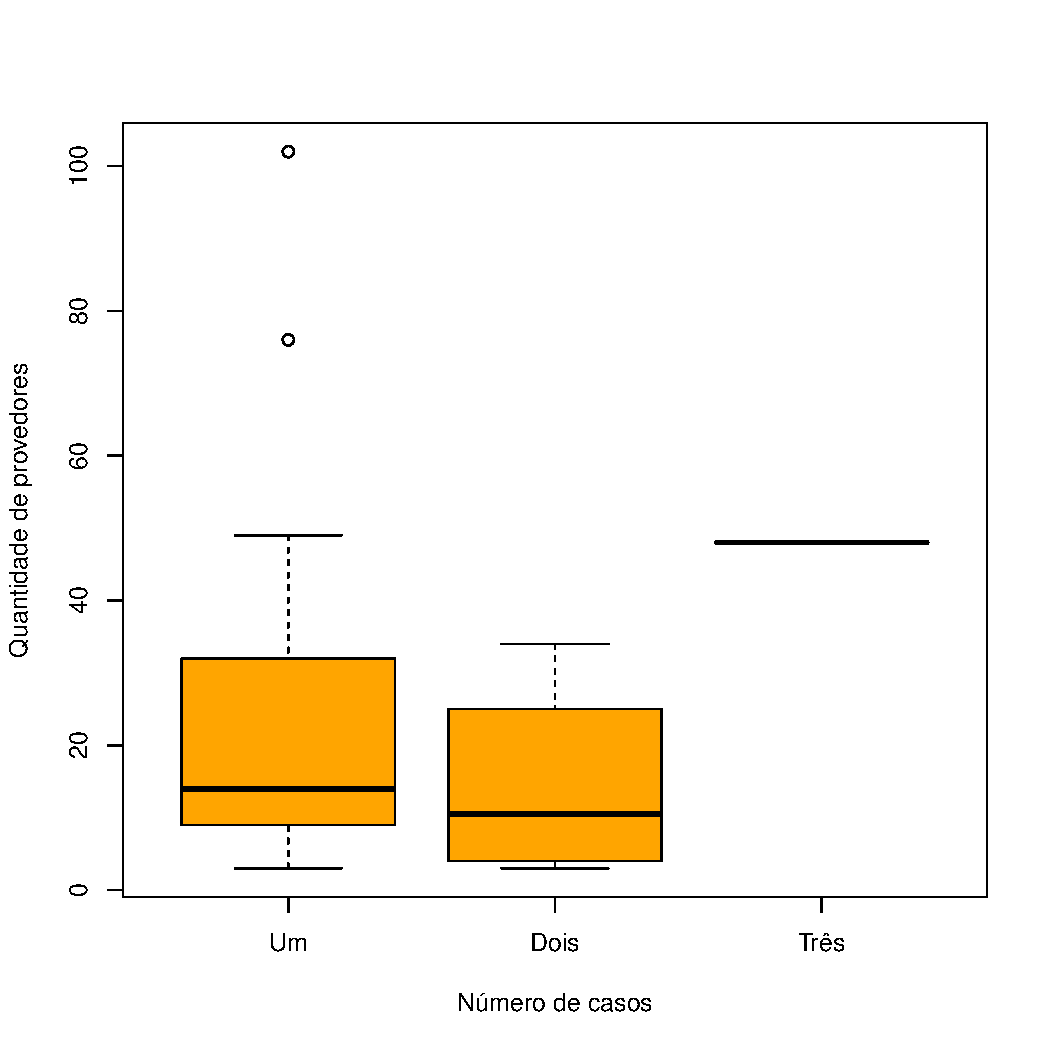
\includegraphics[scale=0.45]{figuras/result_rq1_once_twice_three_2.pdf}}
    }
    \caption{Quantidade de pacotes/\textit{releases} afetados pelo número de casos de \textit{break change}}
    \label{fig:result_rq1_once_twice_three}
\end{figure}

A Figura \ref{fig:result_rq1_once_twice_three_2} apresenta um \filipe{Vi três boxplots lá} \textit{BoxPlot} da quantidade de provedores que cada pacote possui em relação à quantidade de casos de \textit{break changes} sofridos. O único pacote que foi atingido por três casos de \textit{break change} é o que contém o maior número de \textit{releases} e, mesmo apresentando a menor proporção de casos afetados de acordo com a Figura \ref{fig:result_rq1_once_twice_three_1}, ele possui a maior mediana de provedores que os demais. Nesse caso, três provedores diferentes causaram os três casos de \textit{break changes} e por isso a quantidade de provedores favoreceu a ocorrência dos três casos, uma vez que a quantidade de \textit{releases} não fator determinante, visto a proporção na Figura \ref{fig:result_rq1_once_twice_three_1}. \filipe{Precisa fazer um teste de hipótese e calcular effect size para confirmar o que você está dizendo. Outra coisa é mostrar esse gráfico como um beanplot cortado ao meio. Não acho que o terceiro boxplot seja necessário, só tem um data point nele, não é isso? Dá pra descrever no texto. } Um fato é que a ocorrência de mais de um caso de \textit{break changes} não é tão comum, pois os pacotes que foram atingidos por dois casos possuem uma mediana de provedores menor do que os pacotes que foram atingidos por apenas um caso.

%\subsubsection{Impacto dos provedores indiretos}
%O \gls{npm} contém a maior rede de dependências entre os pacotes dentre os principais repositórios, conforme explicado na Seção \ref{ref-teo:npm}. Nesse emaranhado de projetos dependendo mutuamente uns dos outros, não é difícil pressupor que não somente os provedores diretos podem introduzir as \textit{break changes}. Assim como o cliente usa o provedor direto, o provedor indireto é usado da mesma maneira pelo provedor direto, fazendo do provedor indireto um indivíduo muito influente para a execução do cliente.

\section{RQ2. Como os pacotes provedores introduzem \textit{breaking changes} em uma \textit{release}?}


\subsubsection{Categorias de \textit{Break changes}}
A linguagem \textit{Javascript} é uma linguagem fracamente tipada e dinâmica. Por esse motivo, os códigos escritos nessa linguagem pode apresentar comportamentos diferentes quando comparada com outras linguagens. Por isso há a necessidade de se conhecer as  categorias de \textit{break changes} que são encontradas no ecossistema do \gls{npm}. Assim, cada caso de \textit{break change} foi analisada e observado o motivo de seu surgimento e categorizada com as demais. \filipe{Isso é motivação e você já descreveu}

Ao todo, foram 43 casos de \textit{break changes} distribuídas em 39 pacotes \filipe{Uma coisa que você precisa ajeitar ao longo de todo o texto é dizer ``pacote cliente'' e ``pacote provedor''. Aqui está se falando de provedor, mas na seção passada era sobre cliente.}. Todos esses casos foram agrupados em 8 diferentes categorias das quais se encaixavam. A Tabela \ref{tab:bc_category} apresenta cada uma dessas categorias, bem como a quantidade de pacotes e a quantidade de \textit{releases} que cada categoria atingiu.

\begin{table}[]
\begin{tabular}{|l|c|c|c|c|}
\hline
\centering
\textbf{Categoria}           & \textbf{Pacotes afetados} & \textbf{\%}   & \textbf{\textit{Release} afetadas} & \textbf{\%}    \\ \hline
Alteração de regras          & 12              & 27,9 & 64                          & 33,68 \\
Provedores incompatíveis     & 8               & 18,6 & 30                          & 15,78 \\
Alteração de tipo de objeto  & 8               & 18,6 & 24                          & 12,63 \\
Objeto indefinido            & 4               & 9,3  & 25                          & 13,15 \\
Código errado                & 4               & 9,3  & 13                          & 6,84  \\
Código não-atualizado        & 3               & 6,97 & 25                          & 13,15  \\
Renomeação de função         & 3               & 6,97 & 5                           & 2,63  \\
Arquivo não encontrado       & 1               & 2,32 & 4                           & 2,1  \\ \hline
\textbf{Total}               & 43              &      & 190                         &       \\ \hline
\end{tabular}
\caption{Categorias dos casos de \textit{break change}}
\label{tab:bc_category}
\end{table}
\filipe{Muito bom}
A seguir, encontra-se uma descrição sobre cada categoria e um exemplo de como os pacotes dessa determinada categoria foram afetadas.

\begin{itemize}
    \item \textbf{Alteração de regras}: este caso foi o principal que impactou os pacotes. Essa categoria contém os casos de \textit{break change} no qual os provedores possuíam um determinado comportamento, mas alteraram algumas de suas regras/funcionalidades e impactaram os seus clientes. Não foi uma simples alteração no código, tal como uma alteração de tipo de variáveis, ou um código escrito de maneira errada, mas sim uma regra no qual o cliente tinha como sólida, foi alterada. Por exemplo, o pacote \textit{request@2.18.0} introduziu uma alteração em seu código\footnote{https://github.com/request/request/commit/d05b6ba72702c2411b4627d4d89190a5f2aba562\#diff-168726dbe96b3ce427e7fedce31bb0bcR857}, como pode ser visto na Figura \ref{fig:bc_category_change_rule_1}.

    \begin{figure}
        \centering
        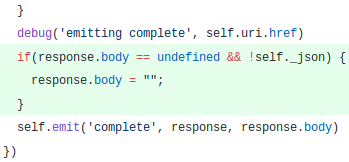
\includegraphics[scale=0.6]{figuras/bc_category_change_rule_1.png}
        \caption{Alteração de regra de funcionamento do \textit{request}}
        \label{fig:bc_category_change_rule_1}
    \end{figure}{}

    Nesse caso, o \textit{request} adiciona uma \textit{string} vazia ao invés de manter \textit{undefined} o corpo de uma requisição. Esse caso do \textit{request} ocorreu exatamente como foi explicado por \citeonline{Foo:2018:ESC:3236024.3275535} dizendo que os pacotes evoluem independentemente dos clientes. Essa alteração na regra do \textit{request} reflete em uma evolução do pacote, mas o cliente não esperava essa alteração e confiava que o corpo da resposta fosse retornado como \textit{undefined} em caso de erro, por isso o cliente quebrou.

    \item \textbf{Provedores incompatíveis}: nessa categoria, há um provedor direto A e um provedor indireto B envolvido, o qual alterou o seu código, o que não gerou um erro, mas provocou no provedor A um comportamento inesperado, ou seja, o provedor B passou a ser incompatível com o provedor A. Nessa categoria, nenhum dos provedores contém um erro, mas sim uma incompatibilidade. Um exemplo disso ocorreu com os pacotes \textit{babel-eslint}\footnote{https://www.npmjs.com/package/babel-eslint} e \textit{escope}\footnote{https://www.npmjs.com/package/escope}, entretanto, o pacote \textit{escope} é um provedor indireto do \textit{babel-eslint}.

    \begin{figure}
        \centering
        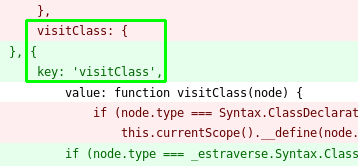
\includegraphics[scale=0.5]{figuras/bc_category_incompatibles_providers.png}
        \caption{Alteração de código do \textit{escope}}
        \label{fig:bc_category_incompatibles_providers}
    \end{figure}{}

    A \textit{releases escope@3.4} realizou uma alteração no seu código, de acordo com a Figura \ref{fig:bc_category_incompatibles_providers}, mas que não reflete em um erro. Essa alteração impactou diretamente o pacote \textit{babel-eslint}, mesmo o pacote \textit{escope} não sendo um provedor direto do \textit{babel-eslint} e não ter introduzido um erro\footnote{https://github.com/estools/escope/issues/99\#issuecomment-178151491}. Com isso, há uma incompatibilidade entre os provedores e essa incompatibilidade precisou ser corrigida pelo \textit{babel-eslint} e não pelo \textit{escope}. Essa foi a \textit{break change} que mais surgiu na análise manual pois, dos 43 casos, 5 (11.6\%) refletiam essa incompatibilidade, uma vez que o \textit{babel-eslint} é provedor de 5.8\% de toda a base de dados.

    \item \textbf{Alteração de tipo de objeto}: essa é uma categoria de \textit{break changes} facilmente detectável em linguagens fortemente tipadas, mas no \textit{Javascript} representam um tipo de \textit{break change} que, por muitas vezes, pode nem afetar o código do cliente. Mas, neste trabalho, foram detectados 8 (18.6\%) de casos nos quais os provedores alteraram o tipo de alguma variável.

    \begin{figure}
        \centering
        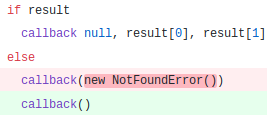
\includegraphics[scale=0.5]{figuras/bc_category_change_type.png}
        \caption{Alteração de um tipo \textit{array} para \textit{object}}
        \label{fig:bc_category_change_type}
    \end{figure}{}

    Na Figura \ref{fig:bc_category_change_type} o provedor \textit{socket.io}\footnote{https://www.npmjs.com/package/socket.io} alterou alguns \textit{arrays} para \textit{object}\footnote{https://github.com/socketio/socket.io/commit/b73d9bea4efb48277eee685763026ff2df5a79ab}. Anteriormente, os clientes iteravam nesses \textit{arrays}, mas após essa alteração, os clientes foram afetados.

    \item \textbf{Objeto indefinido}: por vezes, os códigos podem estar todos corretos, mas então o provedor tenta acessar uma variável que não existe. Esta categoria de \textit{break change} representa os casos no qual os provedores tentaram obter acesso à alguma variável/objeto, mas que não existiam. Esses erros são os que facilmente podem ser consertados/evitados apenas adicionando o código da Listagem \ref{cod:undefined_object}:

    \begin{lstlisting}[style=bash, label=cod:undefined_object]
    this.var = this.var || {};
    \end{lstlisting}

    Esse tipo de erro surgiu no pacote \textit{ember-cli-htmlbars-inline-precompile}\footnote{https://www.npmjs.com/package/ember-cli-htmlbars-inline-precompile}, no qual o desenvolvedor tenta acessar uma variável que não estava disponível. Mas, assim como o desenvolvedor já havia feito com as demais variáveis da Figura \ref{fig:bc_category_undefined_object}, uma simples alteração no código foi o suficiente.

    \begin{figure}
        \centering
        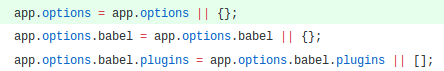
\includegraphics[scale=0.7]{figuras/bc_category_undefined_object.png}
        \caption{Correção do erro de objeto indefinido}
        \label{fig:bc_category_undefined_object}
    \end{figure}{}

    \item \textbf{Código errado}: este caso de \textit{break change} ocorreu quando o provedor escreveu um código semanticamente incorreto, gerando um erro na sua execução e afetando o cliente. Em linguagens compilada, esse tipo de erro seria facilmente identificado pelo compilador em tempo de compilação. Foi exatamente isso que a dependência fez. Ao alterar o seu código, o desenvolvedor escreveu duas vezes a mesma variável, como pode ser visto na Figura \ref{fig:bc_category_wrong_code}. Assim como os erros do tipo \textit{undefined object}, os erros dessa categoria  são facilmente corrigidos.

    \begin{figure}
        \centering
        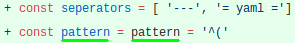
\includegraphics[scale=0.8]{figuras/bc_category_wrong_code.png}
        \caption{Código semanticamente incorreto}
        \label{fig:bc_category_wrong_code}
    \end{figure}{}

    \item \textbf{Renomeação de função}: as \textit{break changes} relacionadas à esta categoria foram facilmente detectáveis. Quando a mensagem de erro do \textit{node.js} era exibida como \textit{TypeError: var is not a function}, com pouca investigação já era possível saber que uma determinada função não estava mais disponível, ou seja, havia sido removida ou alterado o seu nome.

    \begin{figure}
        \centering
        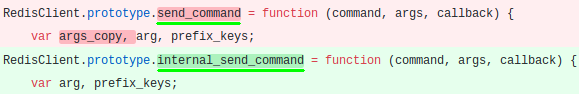
\includegraphics[scale=0.6]{figuras/bc_category_renamed_function.png}
        \caption{Alteração do nome de função}
        \label{fig:bc_category_renamed_function}
    \end{figure}{}

    \item \textbf{Arquivo não encontrado}: os casos de \textit{break change} relacionados à esta categoria são aqueles no qual o desenvolvedor realiza um acesso a um arquivo, mas esse não existe. O arquivo requerido pode não existir ou não estar disponível, uma vez que, referenciado no arquivo \textit{.npmignore} -- arquivo utilizado pelo \textit{npm} para ignorar arquivos durante o processo de publicação --, o arquivo existe mas não está disponível, mas também o arquivo pode não existir. Entretanto, o único caso de arquivo não encontrado ocorreu pois o arquivo \textit{index.js} estava indisponível. O provedor \textit{esprima-extract-comments}\footnote{https://www.npmjs.com/package/esprima-extract-comments} utilizava como provedor um \textit{fork} do pacote \textit{esprima}\footnote{https://github.com/ariya/esprima/} e o referencia em seu  \textit{package.json} para ser descarregado diretamente do \textit{Github}\footnote{https://github.com/jonschlinkert/esprima-extract-comments/blob/6b65a0f52f85bc6fa830d44e352ec3da9e9ef620/package.json\#L47}. Entretanto, o \textit{index.js} desse \textit{fork}, foi referenciado no \textit{.gitignore} e não estava disponível quando o \textit{npm} descarregou o pacote diretamente do \textit{Github}, mas o arquivo estava disponível se o pacote \textit{exprima} fosse descarregado diretamente do \textit{npm}.

\end{itemize}{}

\filipe{Muito bom}

\section{RQ3. Como os pacotes clientes se recuperam das \textit{breaking changes}?}